\section{Metodología}
En esta sección presenta una propuesta para evaluar la precisión de modelos de regresión lineal mediante intervalos de confianza para el coeficiente de determinación \(R^2\). Se consideran modelos Exactos-Precisos (EP) y Exactos-Imprecisos (EI) bajo diferentes supuestos: Normalidad-Varianza Constante (NVC), No Normalidad-Varianza Constante (NNVC), Normalidad-Varianza Distinta (NVD) y No Normalidad-Varianza Distinta (NNVD). Se aplican esquemas de Bootstrap, incluyendo algoritmos de \textcite{wu-1986}, \textcite{liu-1988}, \textcite{zacarias-2023} y \textcite{balam-2012}, utilizando distintas técnicas de remuestreo y estimadores robustos según el cumplimiento de supuestos.\\

La metodología se valida mediante la simulación de 24,000 modelos distribuidos en 48 escenarios, cada uno con 500 modelos y 5 réplicas. Se consideran factores como el tamaño de muestra, precisión y supuestos. Se construyen intervalos Bootstrap (Percentil y BCa) para determinar la precisión de \(R^2\), evaluando su eficacia mediante la frecuencia con la que los intervalos contienen el valor verdadero y analizando su ancho. Se realiza un análisis ANOVA factorial para identificar diferencias significativas entre los intervalos, complementado con pruebas de Tukey. Las simulaciones y análisis se implementan en el lenguaje R.


\subsection{Una Propuesta para Evaluar la Precisión de un Modelo}

En esta propuesta para evaluar la precisión de un modelo se considera: el conocimiento del tipo de caso de esté ante los cuatro escenarios posibles bajo el cumplimiento de los supuestos de normalidad y/o varianza contante, los predichos $(z)$, los observados $(y)$ para generar muestras Bootstrap del coeficiente de determinación $R^{2}$. Se propone construir intervalos de confianza con el método Percentil y BCa a través de las muestras obtenidas, por ocho esquemas Bootstrap. \\ 

\subsubsection{Estimadores y Esquemas Bootstrap}

Se debe considerar tres tipos de casos bajo el cumplimiento de los supuestos de normalidad y/o varianza contante:

\begin{description}
	\item[] Caso - 1 NVC
	\item[] Caso - 2 NNVC
	\item[] Caso - 3 NVD \& NNVD
\end{description}


Es necesario construir los intervalos de confianza con los métodos: Percentil y BCa para la $R^{2}$. Dado el desconocimiento de la función de distribución del coeficiente de determinación, se propone el uso de los esquemas Bootstrap propuestos en \textcite{rana-2012} e implementados en \textcite{zacarias-2023}, al igual de los dos esquemas Bootstrap implementados en \textcite{balam-2012}. Dependiendo el caso a evaluar se utiliza los estimadores de mínimos cuadrados o el MM-estimador robusto.\\


\textit{Estimador de mínimos cuadrados para el Caso 1- NVC.}. En este caso se propone utilizar los estimadores al correr una regresión simple, junto a los residuales y los valores ajustados $\hat{y}$ obtenido por la regresión.\\


\textit{MM-estimador para el Caso 2- NVC y  Caso - 3 NVD \& NNVD}. En ambos casos se propone utilizar el MM-estimador con regresión robusta junto con los residuales robustos y los valores ajustados $\hat{y}$ robustos obtenidos por la regresión. Para el Caso 2- NVC, los residuales robustos se utilizaran sin ponderar y para el  Caso - 3 NVD \& NNVD los residuales robustos se ponderaran.  \\



\textit{Bootstrap robusto y Bootstrap de Residuales Balanceados para todos los casos}. Para todos los casos se propone utilizar siete esquemas Bootstrap a los residuales dependiendo sus caso, los siguientes esquemas robustos: los tres de Wu , los dos de Liu y el Robusto simple. Adicionalmente, se propone implementar justo a los seis esquemas robustos, el Bootstrap de Residuales Balanceados. \\


\textit{Bootstrap Pareado Balanceado para todos los casos}. El \textit{Algoritmo de pareado} al aplicar el remuestreo sobre una muestra pareada de las observaciones con su respectiva predicha y no depender de los estimadores al uno utilizar los residuales, se implementa sin importar el tipo de caso, con las $z$ y $y$ proporcionadas.\\

Este proceso que permite desarrollar los esquemas Bootstrap dependiendo del caso del modelo se encuentra descrito en la Figura ~\ref{fig:AlgDifEsqBoots}

 

\begin{figure}
	\centering 
	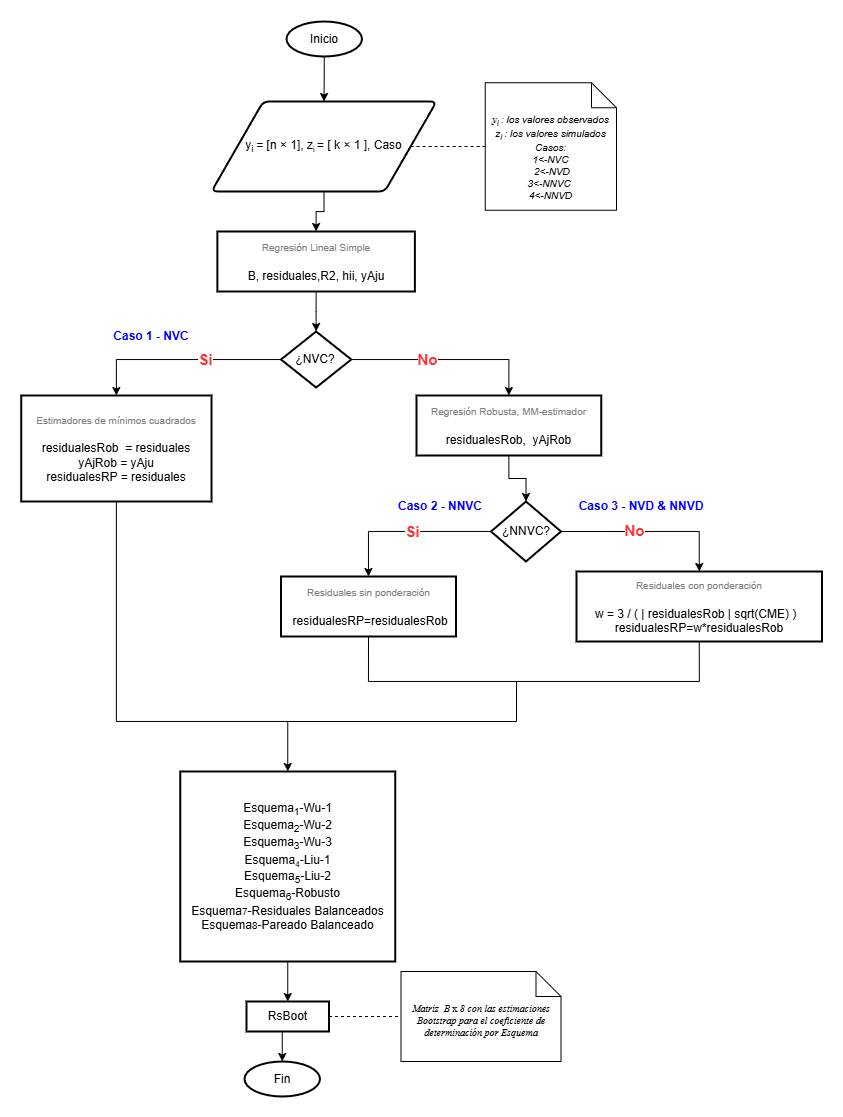
\includegraphics[width=0.4\linewidth]{img/metodologia_v4.png} 
	\caption{Algoritmo para los diferentes esquemas Bootstrap.}
	\label{fig:AlgDifEsqBoots}
\end{figure}

\subsubsection{Intervalos de Confianza para la $R^{2}$}

Para evaluar la precisión del modelo se propone utilizar los intervalos de confianza Percentil y BCa para cada una de las muestras de $R^{2}s$ obtenidas en el procedimiento anterior por esquema Bootstrap. Para ello se realizan las siguientes modificaciones a los algortimos de percentil y BCa: \\


\textbf{Algoritmo - Intervalo de Confianza Percentil}

\begin{enumerate}
	
	\item Se obtienen las muestras $\hat{R}^{2*}_{1} , \hat{R}^{2*}_{2}, \dots,\hat{R}^{2*}_{B}$.
	
	\item Las $B$ muestras $\hat{R}^{2*}_{1} , \hat{R}^{2*}_{2}, \dots,\hat{R}^{*}_{B}$ se ordenan de manera ascendente, tal que $\hat{R}^{2*}_{1} \leq \hat{R}^{2*}_{2} \leq \dots \leq \hat{R}^{2*}_{B} $.
	
	\item Determinar los cuantiles \( LI_{P} \) y \( LS_{P} \), para el nivel de confianza del \( (1-\alpha)\% \) en la muestra ordenada, con \( LI_{P} = \hat{R}^{2*}_{ ( \alpha/2 ) \times B} \) y \( LS_{P} = \hat{R}^{2*}_{ (1 - \alpha/2) \times B} \).
	
	\item El intervalo de confianza está dado por: \( [LI_{P}, LS_{P}] \).
\end{enumerate}


\textbf{Algoritmo - Intervalo de Confianza BCa}

\begin{enumerate}
	
	\item Se obtienen las muestras $\hat{R}^{2*}_{1} , \hat{R}^{2*}_{2}, \dots,\hat{R}^{2*}_{B}$.
	
	\item Obtener la estimación de $\hat{R}^{2}$ a partir de los datos originales con una regresión lineal simple.
	
	\item Se determina la proporción $p$ de las  $\hat{R}^{2*}_{i}$ que son mayores o iguales a $\hat{R}^{2}$.
	
	\item  Determinar $Z_{0} = Z_{p}$ donde $Z_{p}$ es el cuantil en la distribución normal estándar tal que $P(Z > Z_{p}) = p$.
	
	\item  Obtener la constante de aceleración $a$ dada por:
	\begin{center}
		\Large $ a = \frac{\sum_{i=1}^{n}  (\hat{R}^{2}_{-iprom}  - \hat{R}^{2}_{-i})^{3} }{ 6 \; (\; \sum_{i=1}^{n}  ( \hat{R}^{2}_{-iprom}  - \hat{R}^{2}_{-i} \;)^{2} \; )^{3/2}} $
	\end{center}
	
	donde: $\hat{R}^{2}_{-i}$ es la estimación con los datos originales quitando la $i$-esima observación y {\normalsize $\hat{R}^{2}_{-iprom} = \frac{1}{n} \sum_{i=1}^{n}\hat{R}^{2}_{-i}$}
	
	\item Obtener {\large $Z_{L} = \frac{Z_{0} - Z_{\alpha/2}}{ 1- \alpha ( Z_{0} - Z_{\alpha/2})} + Z_{0}  $}   y {\large $Z_{U} = \frac{Z_{0} + Z_{\alpha/2}}{ 1- \alpha ( Z_{0} - Z_{\alpha/2})} + Z_{0}  $}  donde: $Z_{\alpha /2}$ es el cuantil en la
	distribución normal estándar tal que $P(Z > Z_{\alpha / 2}) = \frac{\alpha}{2}$.
	
	\item Determinar \( LI_{BCa} = \text{INVCDF}(\Phi(Z_{L})) \) y \( LS_{BCa} = \text{INVCDF}(\Phi(Z_{U})) \), donde \( \text{INVCDF} \) es el cuantil en la muestra Bootstrap \( \hat{R}^{2*}_{1}, \hat{R}^{2*}_{2}, \dots, \hat{R}^{2*}_{B} \) con probabilidad \( \Phi(Z_{L}) \) y \( \Phi(Z_{U}) \) respectivamente.
	
	\item El intervalo de confianza está dado por: \( [LI_{BCa}, LS_{BCa}] \).

\end{enumerate}




A continuación se describe el algoritmo para evaluar la precisión de un modelo construyendo intervalos de confianza para cada esquema Bootstrap:\\


\textbf{Algoritmo para Evaluar la Precisión de un Modelo}

\begin{enumerate}
	
	\item Llamar la función y aplicar el algoritmo con los esquemas Bootstrap para generar la matriz \( \mathbf{RsBoot} \) de orden \( b \times k \), donde:
	\begin{itemize}
		\item \( b \) es el número de remuestras generadas (\( \hat{R}^{2*}_{1}, \hat{R}^{2*}_{2}, \dots, \hat{R}^{2*}_{b} \)).
		\item \( k \) es el número de esquemas Bootstrap considerados (\( k = 8 \)).
	\end{itemize}
	
	\item Para cada columna \( k \) (\( k = 1, 2, \dots, 8 \)) en la matriz de remuestras \( RsBoot \):
	\begin{itemize}
		\item Construir el intervalo de confianza Percentil \( [LI_{P_k}, LS_{P_k}] \) utilizando el Algoritmo Percentil.
		\item Construir el intervalo de confianza BCa \( [LI_{BCa_k}, LS_{BCa_k}] \) utilizando el Algoritmo BCa.
	\end{itemize}
\end{enumerate}




















	 
	 
\subsection{Estudio de simulación para la evaluación de la propuesta}
\vspace{1.5cm}

\subsubsection{Simulación de modelo}
Simular modelos exactos-precisos (EP) y modelos exactos-imprecisos (EI) mediante la propuesta de Febles (2014) y Zacarías (2023); cuando se cumplan o no los supuestos de normalidad e igualdad de varianzas.

%aqui va el diagrama
Diseñar e implementar un estudio de simulación para evaluar la eficacia de la metodología propuesta.
	 \vspace{1.5cm}
	 	 
	 	 
	 	 
	 	 
\subsection{Análisis estadísticos}
Para cada supuesto (NVC, NNVC, NVD, NNVD) se utilizó ANOVA en un arreglo factorial de tres factores seguido de la comparación múltiple de Tukey (Montgomery, 2017), para determinar el comportamiento de la eficacia de dos ICB en la evaluación de la precisión, bajo ocho esquemas de remuestreo, seis tamaños de muestra y dos tipos de modelo. Cabe señalar que, en cuatro de los ocho análisis de varianza realizados se eliminaron valores atípicos para el logro del cumplimiento de los supuestos del ANOVA.
Las pruebas estadísticas se consideraron significativas cuando  y se utilizó el paquete estadístico STATGRAPHICS Centurion 19 (Statgraphics, 2024).




